\begin{figure}[!htbp]\centering
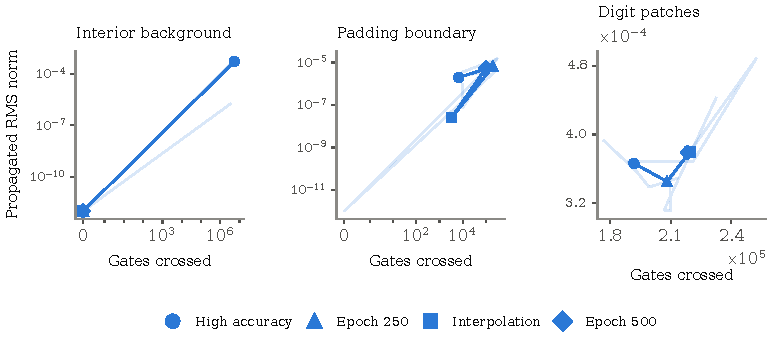
\includegraphics[width=4.629in]{background_trajectory.pdf}
\caption{Conv1 gate crossings and propagated residuals in the base MNIST CNN at layer-relative radius $0.01$. Each point is a training stage: within-seed medians over 128 matched directions, then means over three seeds; faint paths show individual seeds. Paths follow training order. Background and boundary panels use a horizontal scale linear up to one crossing and logarithmic above it; the digit panel uses linear axes to resolve its narrower range. Zero propagated contributions are drawn at $10^{-12}$.}\label{fig:c-cnn-background}
\end{figure}
\FloatBarrier
